\chapter{Музыкальные композиции}
\label{ch:musical-composition}
Статья посвящена исследованию музыкальных композиций на основе базы знаний международного проекта Викиданные. С помощью SPARQL-запросов, вычисляемых на объектах типа <<музыкальная композиция>> в Викиданных, получен список всех музыкальных композиций, список музыкальных композиций, имеющих композиторов, а также построена пузырьковая диаграмма, показывающая композиторов с наибольшим количеством композиций. Кроме того, решена задача поиска музыкальных лакун в общественном достоянии и выполнена оценка полноты Викиданных.

\section{Экземпляры объекта <<Музыкальные композиции>>}

\marginnote{Используемые в запросах объекты: \wdqName {<<музыкальное произведение/композиция>>} {105543609};
Используемое свойство: \wdProperty{31}{<<экземпляр>>}}

Построим список всех музыкальных композиций.

\begin{lstlisting}[ language=SPARQL,
                    caption={\href{https://w.wiki/5$CG}{Список всех  музыкальных композиций}\protect\footnotemark},
                    label=lst:musical_composition,
                    texcl 
                    ]
#List of all musical compositions
SELECT ?composition ?compositionLabel 
WHERE {
  ?composition wdt:P31 wd:Q105543609.
  SERVICE wikibase:label { bd:serviceParam wikibase:language "ru,en". }
}
\end{lstlisting}%
\footnotetext{Получено: \num{5495} записи на 2017 год. Ссылка на SPARQL-запрос: \href{https://w.wiki/5$CG}{https://w.wiki/5$CG}.}

Наиболее полными и проработанными музыкальными композициями на Викиданных являются: \wdqName{Волшебная флейта}{5064}, \wdqName{К Элизе}{11980}, \wdqName{Реквием}{207875}, \wdqName{Маленькая ночная серенада}{12025}.

Почти пустыми и малоинформативными музыкальными композициями были: \wdqName{Полёт шмеля}{1342275}, \wdqName{Ромео и Джульетта}{763716}, \wdqName{Симфонический эпизод «Завод»}{1845909}, \wdqName{Binks’ Waltz}{28807544}, \wdqName{The Rose-bud March}{28803595}, \wdqName{Leola}{28804177}.

В 2022 году тот же скрипт нашёл \num{106757} музыкальных композиций вместо \num{5,5} тысяч в 2017 году. Увеличение числа композиций связано с тем, что эти объекты Викиданных являются теперь не экземплярами объекта «музыкальные произведения», а его экземплярами различных подклассов «музыкального произведения». При поиске подклассов объекта «музыкальные произведения» можно найти такие жанры: \wdqName{драматико-музыкальное произведение}{58483083}, \wdqName{гимн}{484692}, \wdqName{баллада}{182659}.

Найдём количество музыкальных композиций в каждом жанре с помощью следующего запроса.

\begin{lstlisting}[ language=SPARQL,
                    caption={\href{https://w.wiki/5$BV}{ Количество музыкальных композиций в каждом подклассе}\protect\footnotemark},
                    label=lst:music _in_each_subclass,
                    texcl 
                    ]
# Count of pieces of music in each subclass
SELECT ?type (COUNT(?typeInstance) AS ?count) ?typeLabel WHERE {
  ?type wdt:P279* wd:Q105543609.      # subclass of musical composition
  ?typeInstance wdt:P31 ?type  # instance  of that class of which this subject is a particular example and member
  SERVICE wikibase:label { bd:serviceParam wikibase:language "ru, en". }
}
GROUP BY ?type ?typeLabel
ORDER BY DESC (?count)
\end{lstlisting}%
\footnotetext{Получено: \num{161} подкласса музыкальных композиций на 2022 год. Ссылка на SPARQL-запрос: \href{https://w.wiki/5$BV}{https://w.wiki/5$BV}.}

Теперь подсчитаем общее суммарное число музыкальных произведений с учётом музыкальных композиций в подклассах. Для этого добавим в наш скрипт команду \lstinline|SUM()| и удалим лишние строки. Получим такой код:

\begin{lstlisting}[ language=SPARQL,
                    caption={\href{https://w.wiki/5$BT}{ Суммарное число музыкальных произведений с учётом музыкальных композиций в подклассах}\protect\footnotemark},
                    label=lst:The_total_number_of_musical_works_for_all_subclasses,
                    texcl,
	         xleftmargin=18pt
                    ]
# The total number of musical works for all subclasses 
SELECT (SUM(?count) AS ?sum) WHERE{
  SELECT (COUNT(?music) AS ?count) WHERE {
    ?type wdt:P279* wd:Q105543609.  # subclass of musical composition
    ?music wdt:P31 ?type  # instance  of that class of which this subject is a particular example and member
  }
}
\end{lstlisting}%
\footnotetext{Получено: \num{145046} музыкальных произведений на 2022 год. Ссылка на SPARQL-запрос: \href{https://w.wiki/5$BT}{https://w.wiki/5$BT}.}

Можно записать этот код еще короче. Переменная \lstinline|?type| нам не нужна, поэтому можно обойтись без неё, а 4 и 5 строки поменяем местами.

\begin{lstlisting}[ language=SPARQL,
                    caption={\href{https://w.wiki/5$BP}{ Суммарное число музыкальных произведений с учётом музыкальных композиций в подклассах}\protect\footnotemark},
                    label=lst:The_total_number_of_musical_works_for_all_subclasses_up,
                    texcl 
                    ]
# The total number of musical works for all subclasses 
SELECT (SUM(?count) AS ?sum) WHERE{
  SELECT (COUNT(?music) AS ?count) WHERE {
    ?music wdt:P31   # instance of
          [ wdt:P279* wd:Q105543609 ]. # subclass of musical composition
  }
}
\end{lstlisting}%
\footnotetext{Получено: \num{145046} музыкальных произведений на 2022 год. Ссылка на SPARQL-запрос: \href{https://w.wiki/5$BP}{https://w.wiki/5$BP}.}

По сравнению с 2017 годом \num{5494} записи, число записей увеличилось в несколько раз. Это связано с тем, что за 5 лет было добавлено множество новых музыкальных произведений, а также старых, которые не учли ранее.


\subsection{Количество музыкальных произведений по годам}
Далее представлен запрос, подсчитывающий сколько музыкальных произведений было написано в каждом десятилетии с XIX века до настоящего времени.

\begin{lstlisting}[ language=SPARQL,
                    caption={\href{https://w.wiki/7wHy}{ Количество музыкальных композиций за каждые 10 лет}\protect\footnotemark},
                    label=lst:The_number_of_musical_compositions_for_every_10_years,
                    texcl 
                    ]
# The number of musical compositions for every 10 years
#defaultView:BarChart
SELECT (STR(?date) AS ?date_str) (COUNT(?composition) AS ?count) WHERE {
  ?composition wdt:P31 wd:Q105543609;     # instance of compostion
    wdt:P86 ?composer;                    # composition has a composer
    wdt:P577 ?publication.                # composition has a publication date
  BIND(YEAR(?publication) AS ?year)
  BIND((FLOOR(?year / 10 )) * 10  AS ?date)
  FILTER(?publication > "1850-01-01T00:00:00Z"^^xsd:dateTime)
  FILTER(?publication < "2030-01-01T00:00:00Z"^^xsd:dateTime) 
  FILTER (!wikibase:isSomeValue(?publication)) # field "date" must be filled
}
GROUP BY ?date
ORDER BY (?date)
\end{lstlisting}%
\footnotetext{Ссылка на SPARQL-запрос: \href{https://w.wiki/7wHy}{https://w.wiki/7wHy}.}

\begin{marginfigure}[0\baselineskip]
	\includegraphics[width=1\textwidth]{./chapter/musical_composition/BarChart_of_The_number_of_music_compositions_for_every_10_years.svg.png}
	\caption[Гистограмма количества музыкальных композиций за каждые 10 лет с XIX века до настоящего времени]{Гистограмма количества музыкальных композиций за каждые 10 лет с XIX века до настоящего времени}%
\end{marginfigure}
Из графика можно увидеть, что до 1890 года количество написанных музыкальных произведений невелико. После 1890 года начинается резкий подъем и продолжается до нашего времени. Такое увеличение музыкальных произведений можно объяснить тем, что со временем появляются новые жанры и новые устройства для записи. На гистограмме видим два пика: 1960-е — 1980-е (<<первая волна>>), 2000-е и 2010-е (<<вторая волна>>).


\subsection{Количество музыкальных произведений по жанрам}
Найдем, в каких жанрах были написаны музыкальные произведения в пиках графика и изобразим жанры на круговой диаграмме. <<Первая волна>>
\begin{marginfigure}[0\baselineskip]
	\includegraphics[width=1\textwidth]{./chapter/musical_composition/Genre_Chart_1960_—_1980.png}
	\caption[Круговая диаграмма музыкальных жанров за 1960-1980 годы во всем мире]{Круговая диаграмма музыкальных жанров за 1960-1980 годы во всем мире}%
\end{marginfigure}
\begin{lstlisting}[ language=SPARQL,
                    caption={\href{https://w.wiki/6Vx5}{ Количество музыкальных произведений в каждом подклассе}\protect\footnotemark},
                    label=lst:count_of_pieces_of_music_in_each_subclass,
                    texcl 
                    ]
# Count of pieces of music in each subclass
SELECT ?type (COUNT(?typeInstance) AS ?count) ?typeLabel WHERE {
  ?type (wdt:P279*) wd:Q207628.
  ?typeInstance wdt:P31 ?type.
  ?typeInstance wdt:P577 ?publication.
  ?typeInstance wdt:P86 ?composer.
  FILTER(?publication > "1960-01-01T00:00:00Z"^^xsd:dateTime)        
  FILTER(?publication < "1990-01-01T00:00:00Z"^^xsd:dateTime)
  SERVICE wikibase:label { bd:serviceParam wikibase:language "ru, en". }
}
GROUP BY ?type ?typeLabel
ORDER BY DESC (?count)
\end{lstlisting}%
\footnotetext{Ссылка на SPARQL-запрос: \href{https://w.wiki/6Vx5}{https://w.wiki/6Vx5}.}



<<Вторая волна>>

\begin{lstlisting}[ language=SPARQL,
                    caption={\href{https://w.wiki/6Vx6}{ Количество музыкальных произведений в каждом подклассе}\protect\footnotemark},
                    label=lst:count_of_pieces_of_music_in_each_subclass,
                    texcl 
                    ]
# Count of pieces of music in each subclass
SELECT ?type (COUNT(?typeInstance) AS ?count) ?typeLabel WHERE {
  ?type (wdt:P279*) wd:Q207628.
  ?typeInstance wdt:P31 ?type.
  ?typeInstance wdt:P577 ?publication.
  ?typeInstance wdt:P86 ?composer.
  FILTER(?publication > "2000-01-01T00:00:00Z"^^xsd:dateTime)        
  FILTER(?publication < "2020-01-01T00:00:00Z"^^xsd:dateTime)
  SERVICE wikibase:label { bd:serviceParam wikibase:language "ru, en". }
}
GROUP BY ?type ?typeLabel
ORDER BY DESC (?count)
\end{lstlisting}%
\footnotetext{Ссылка на SPARQL-запрос: \href{https://w.wiki/6Vx6}{https://w.wiki/6Vx6}.}

\begin{marginfigure}[0\baselineskip]
	\includegraphics[width=1\textwidth]{./chapter/musical_composition/Genre_Chart_2000-2010.png}
	\caption[Круговая диаграмма музыкальных жанров за 2000-2010 годы во всем мире]{Круговая диаграмма музыкальных жанров за 2000-2010 годы во всем мире}%
\end{marginfigure}

Можем сделать вывод, что жанры музыкальных произведений первого пика, не отличаются от жанров второго. На второй диаграмме, видим сильное преобладание одного жанра <<песня>>. В жанре <<духовная песня>> количество музыкальных произведений уменьшилось. А такие музыкальные жанры как: <<переведенная песня>> и <<лирико-музыкальное произведение>> пропали.

\subsection{Число композиций по десятилетиям в России}
Добавим в скрипт страну происхождения <<Россия>> и <<СССР>>. Ограничение по годам уберем. Получим скрипт, подсчитывающий сколько музыкальных произведений было написано в каждом десятилетии с XIX века до настоящего времени в России и СССР.

\begin{lstlisting}[ language=SPARQL,
                    caption={\href{https://w.wiki/6UUF}{ Количество музыкальных произведений в Росии и СССР за каждые 10 лет}\protect\footnotemark},
                    label=lst:The_number_of_musical_compositions_in_Russia_for_every_10_years,
                    texcl 
                    ]
# The number of musical compositions in Russia for every 10 years
#defaultView:BarChart
SELECT (STR(?date) AS ?date_str) (COUNT(?composition) AS ?count) WHERE {
      {?composition wdt:P17 wd:Q15180}               # country = USSR
  UNION {?composition wdt:P17 wd:Q159}               # country = Russia
  UNION {?composition wdt:P495 wd:Q159}    # country of origin = Russia
  UNION {?composition wdt:P495 wd:Q15180}.  # country of origin =  USSR
  ?composition wdt:P31 wd:Q105543609;     # instance of compostion
    wdt:P86 ?composer;                    # composition has a composer
    wdt:P577 ?publication.                # composition has a publication date

  BIND(YEAR(?publication) AS ?year)
  BIND((FLOOR(?year / 10 )) * 10  AS ?date)
  FILTER (!wikibase:isSomeValue(?publication)) # field "date" must be filled
}
GROUP BY ?date
ORDER BY (?date)
\end{lstlisting}%
\footnotetext{Ссылка на SPARQL-запрос: \href{https://w.wiki/6UUF}{https://w.wiki/6UUF}.}

\begin{marginfigure}[0\baselineskip]
	\includegraphics[width=1\textwidth]{./chapter/musical_composition/Barchart_of_The_number_of_music_compositions_in_Russia_and_USSR_every_10_years.svg.png}
	\caption[Гистограмма количества музыкальных композиций в России и СССР за каждые 10 лет с XIX века до настоящего времени]{Гистограмма количества музыкальных композиций в России и СССР за каждые 10 лет с XIX века до настоящего времени}%
\end{marginfigure}

Количество музыкальных произведений в России и СССР очень мало. Проанализировав несколько песен, написанных в России, таких как: \wdqName {Песня без слов (Кино)} {101001315},  \wdqName{Музыка нас связала} {105724079}, \wdqName {Розовое вино} {57744615}, не попавших в данный скрипт, стало понятно, что у этих произведений отсутствует \wdProperty{495} {Cтрана происхождения}.

\subsection{Поиск музыкальных лакун в общественном достоянии}
Задача состоит в том, чтобы найти такие музыкальные произведения, авторы которых умерли более 70 лет назад, и аудиозапись которых отсутствует на Викискладе. Упорядочить такие произведения от самых старых к новым. Существует практическая выгода и польза от такого скрипта, поскольку видно, какие произведения можно и нужно оцифровывать (с пластинок, кассет) и загружать на Викисклад.

\begin{lstlisting}[ language=SPARQL,
                    caption={\href{https://w.wiki/5$Bf}{ Отсутсвующие аудиозаписи музыкальных произведений, авторы которых умерли более 70 лет назад }\protect\footnotemark},
                    label=lst:music_gaps_in_public_domain,
                    texcl 
                    ]
#Search music gaps in public domain
SELECT ?composition ?compositionLabel ?publication
WHERE {
  ?composition wdt:P31 wd:Q105543609.             # instance of compostion
  ?composition wdt:P86 ?composer.              # composition has a composer
  ?composition wdt:P577 ?publication.          # composition has a publication date
  ?composer wdt:P570 ?death.                   # composer has a date of death
  MINUS {?composition wdt:P51 []}.             # compositions without audio 
  FILTER(?death < "1947-01-01T00:00:00Z"^^xsd:dateTime)        # composers that passed away more than 70 years ago
  FILTER(?publication < "1947-01-01T00:00:00Z"^^xsd:dateTime)  # compositions that were published more thatn 70 years ago
  SERVICE wikibase:label { bd:serviceParam wikibase:language "ru,en". }
}
ORDER BY ASC(?publication)
\end{lstlisting}%
\footnotetext{Получено: \num{3771} записи. Ссылка на SPARQL-запрос: \href{https://w.wiki/5$Bf}{https://w.wiki/5$Bf}.}


\subsection{Полнота Викиданных}
Проанализируем полноту Викиданных.

По данным \href{https://ru.wikipedia.org/wiki/Музыкальный_словарь_Гроува}{<<Музыкального словаря Гроува>>} за всю историю человечества существовало \num{20374} композиторов.

По данным категории \href{https://ru.wikipedia.org/wiki/Категория:Композиторы_по_алфавиту}{<<Композиторы по алфавиту>>} Русской Википедии существует \num{6130} композиторов.

По данным категории \href{https://en.wikipedia.org/wiki/List_of_composers_by_name}{<<List of composers by name>>} Английской Википедии существует \num{4685} композиторов.

Количество музыкальных композиций с заполненным свойством \wdProperty{86}{<<композитор>>} равно \num{3862}, {что показывает нам \href{https://w.wiki/56Rc}{SPARQL-запрос}.}, и это с учётом того, что один композитор мог написать несколько музыкальных произведений. Например, \href{https://ru.wikipedia.org/wiki/Моцарт,_Вольфганг_Амадей}{Вольфганг Амадей Моцарт} написал \num{95} произведений, что существенно снижает количество уникальных композиторов. Полученное число \num{3862} меньше, чем количество композиторов из русской и английской Википедии, и существенно меньше, чем количество композиторов из \href{https://ru.wikipedia.org/wiki/Музыкальный_словарь_Гроува}{<<Музыкального словаря Гроува>>}, что говорит нам о неполноте Викиданных.

\href{https://w.wiki/56Rj}{SPARQL-запрос} по композициям с заполненным свойством \wdProperty{86}{<<композитор>>} и свойством \wdProperty{495}{<<страна происхождения>>}, имеющим значения \wdqName{<<Российская империя>>}{34266}, \wdqName{<<СССР>>}{15180} или \wdqName{<<Россия>>}{159}, выдал всего лишь \num{8} произведений, что говорит о невозможности анализа русских музыкальных произведений в связи с недостатком данных.

Построим пузырьковую диаграмму композиторов музыкальных композиций.

\footnotetext{Получено: \num{773} записи. Ссылка на SPARQL-запрос: \href{https://w.wiki/5$CK}{https://w.wiki/5$CK}.}
\begin{lstlisting}[ language=SPARQL, numbers=none,
                    caption={\href{https://w.wiki/5$CK}{ Пузырьковая диаграммп композиторов музыкальных композиций }\protect\footnotemark},
                    label=lst:BubbleChart,
                    texcl 
                    ]
#composers of musical compositions
#defaultView:BubbleChart
SELECT ?composer ?form (COUNT(*) AS ?count) WHERE {
  ?composition wdt:P31 wd:Q105543609.
  ?composition wdt:P86 ?composer.
  OPTIONAL {
    ?composer rdfs:label ?form.
    FILTER((LANG(?form)) = "ru,en")
  }
}
GROUP BY ?composer ?form
ORDER BY DESC(?count) ?form
\end{lstlisting}%

Запрос ~\ref{lst:BubbleChart} представлен на рис. ~\ref{fig:bubbleChart} и рис. ~\ref{fig:bubbleChart2}.

Размер круга означает количество написанных музыкальных композиций. Диаграмма показывает, что у одних композиторов значительно больше композиций чем у других. В первую пятерку входят \href{https://ru.wikipedia.org/wiki/Гаде,_Нильс}{Нильс Гаде} (\num{173} композиции), \href{https://ru.wikipedia.org/wiki/Бах,_Иоганн_Себастьян}{Иоганн Себастьян Бах} (\num{155} композиций), \href{https://ru.wikipedia.org/wiki/Синдинг,_Кристиан_Август}{Кристиан Август Синдинг} (\num{125} композиций), \href{https://ru.wikipedia.org/wiki/Хальворсен,_Юхан}{Юхан Хальворсен} (\num{121} композиция), \href{https://ru.wikipedia.org/wiki/Хованесс,_Алан}{Алан Хованесс} (\num{108} композиций).

Диаграмма ~\ref{fig:bubbleChart2} за 2022 год позывает как изменилось количество написанных композиций у различный композиторов. По сравнению с 2017 годом в первую пятерку входят \href{https://ru.wikipedia.org/wiki/Маклауд,_Кевин}{Маклауд Кевин} (\num{1237} композиций), \href{https://ru.wikipedia.org/wiki/Гендель,_Георг_Фридрих}{Гендель Георг Фридрих} (\num{1236} композиция), \href{https://en.wikipedia.org/wiki/R._D._Burman}{Рахул Дев Бурман} (\num{744} композиций), \href{https://ru.wikipedia.org/wiki/Моцарт,_Вольфганг_Амадей}{Вольфганг Амадей Моцарт} (\num{699} композиций),\href{https://ru.wikipedia.org/wiki/Люлли,_Жан-Батист}{ Жан-Батист Люлли} (\num{686} композиций). Исходя из данных диаграмм, можно сделать вывод, что появились новые композиторы, которые имеют значительно больше публикаций. Так же можно наблюдать имена старых композиторов, тоже с существенным приростом опубликованных композиций, что говорит о дополнении Викиданных ранее не учтенными произведениями.

\begin{figure*}
	\includegraphics[width=\textwidth]{./chapter/musical_composition/Composer_of_musical_compositions_bubble_diagram.png}
	\caption[Пузырьковая диаграмма композиторов по количеству написанных композиций за 2017 год]{Пузырьковая диаграмма композиторов по количеству написанных композиций за 2017 год}%
 	\label{fig:bubbleChart}%
\end{figure*}
\begin{figure*}
	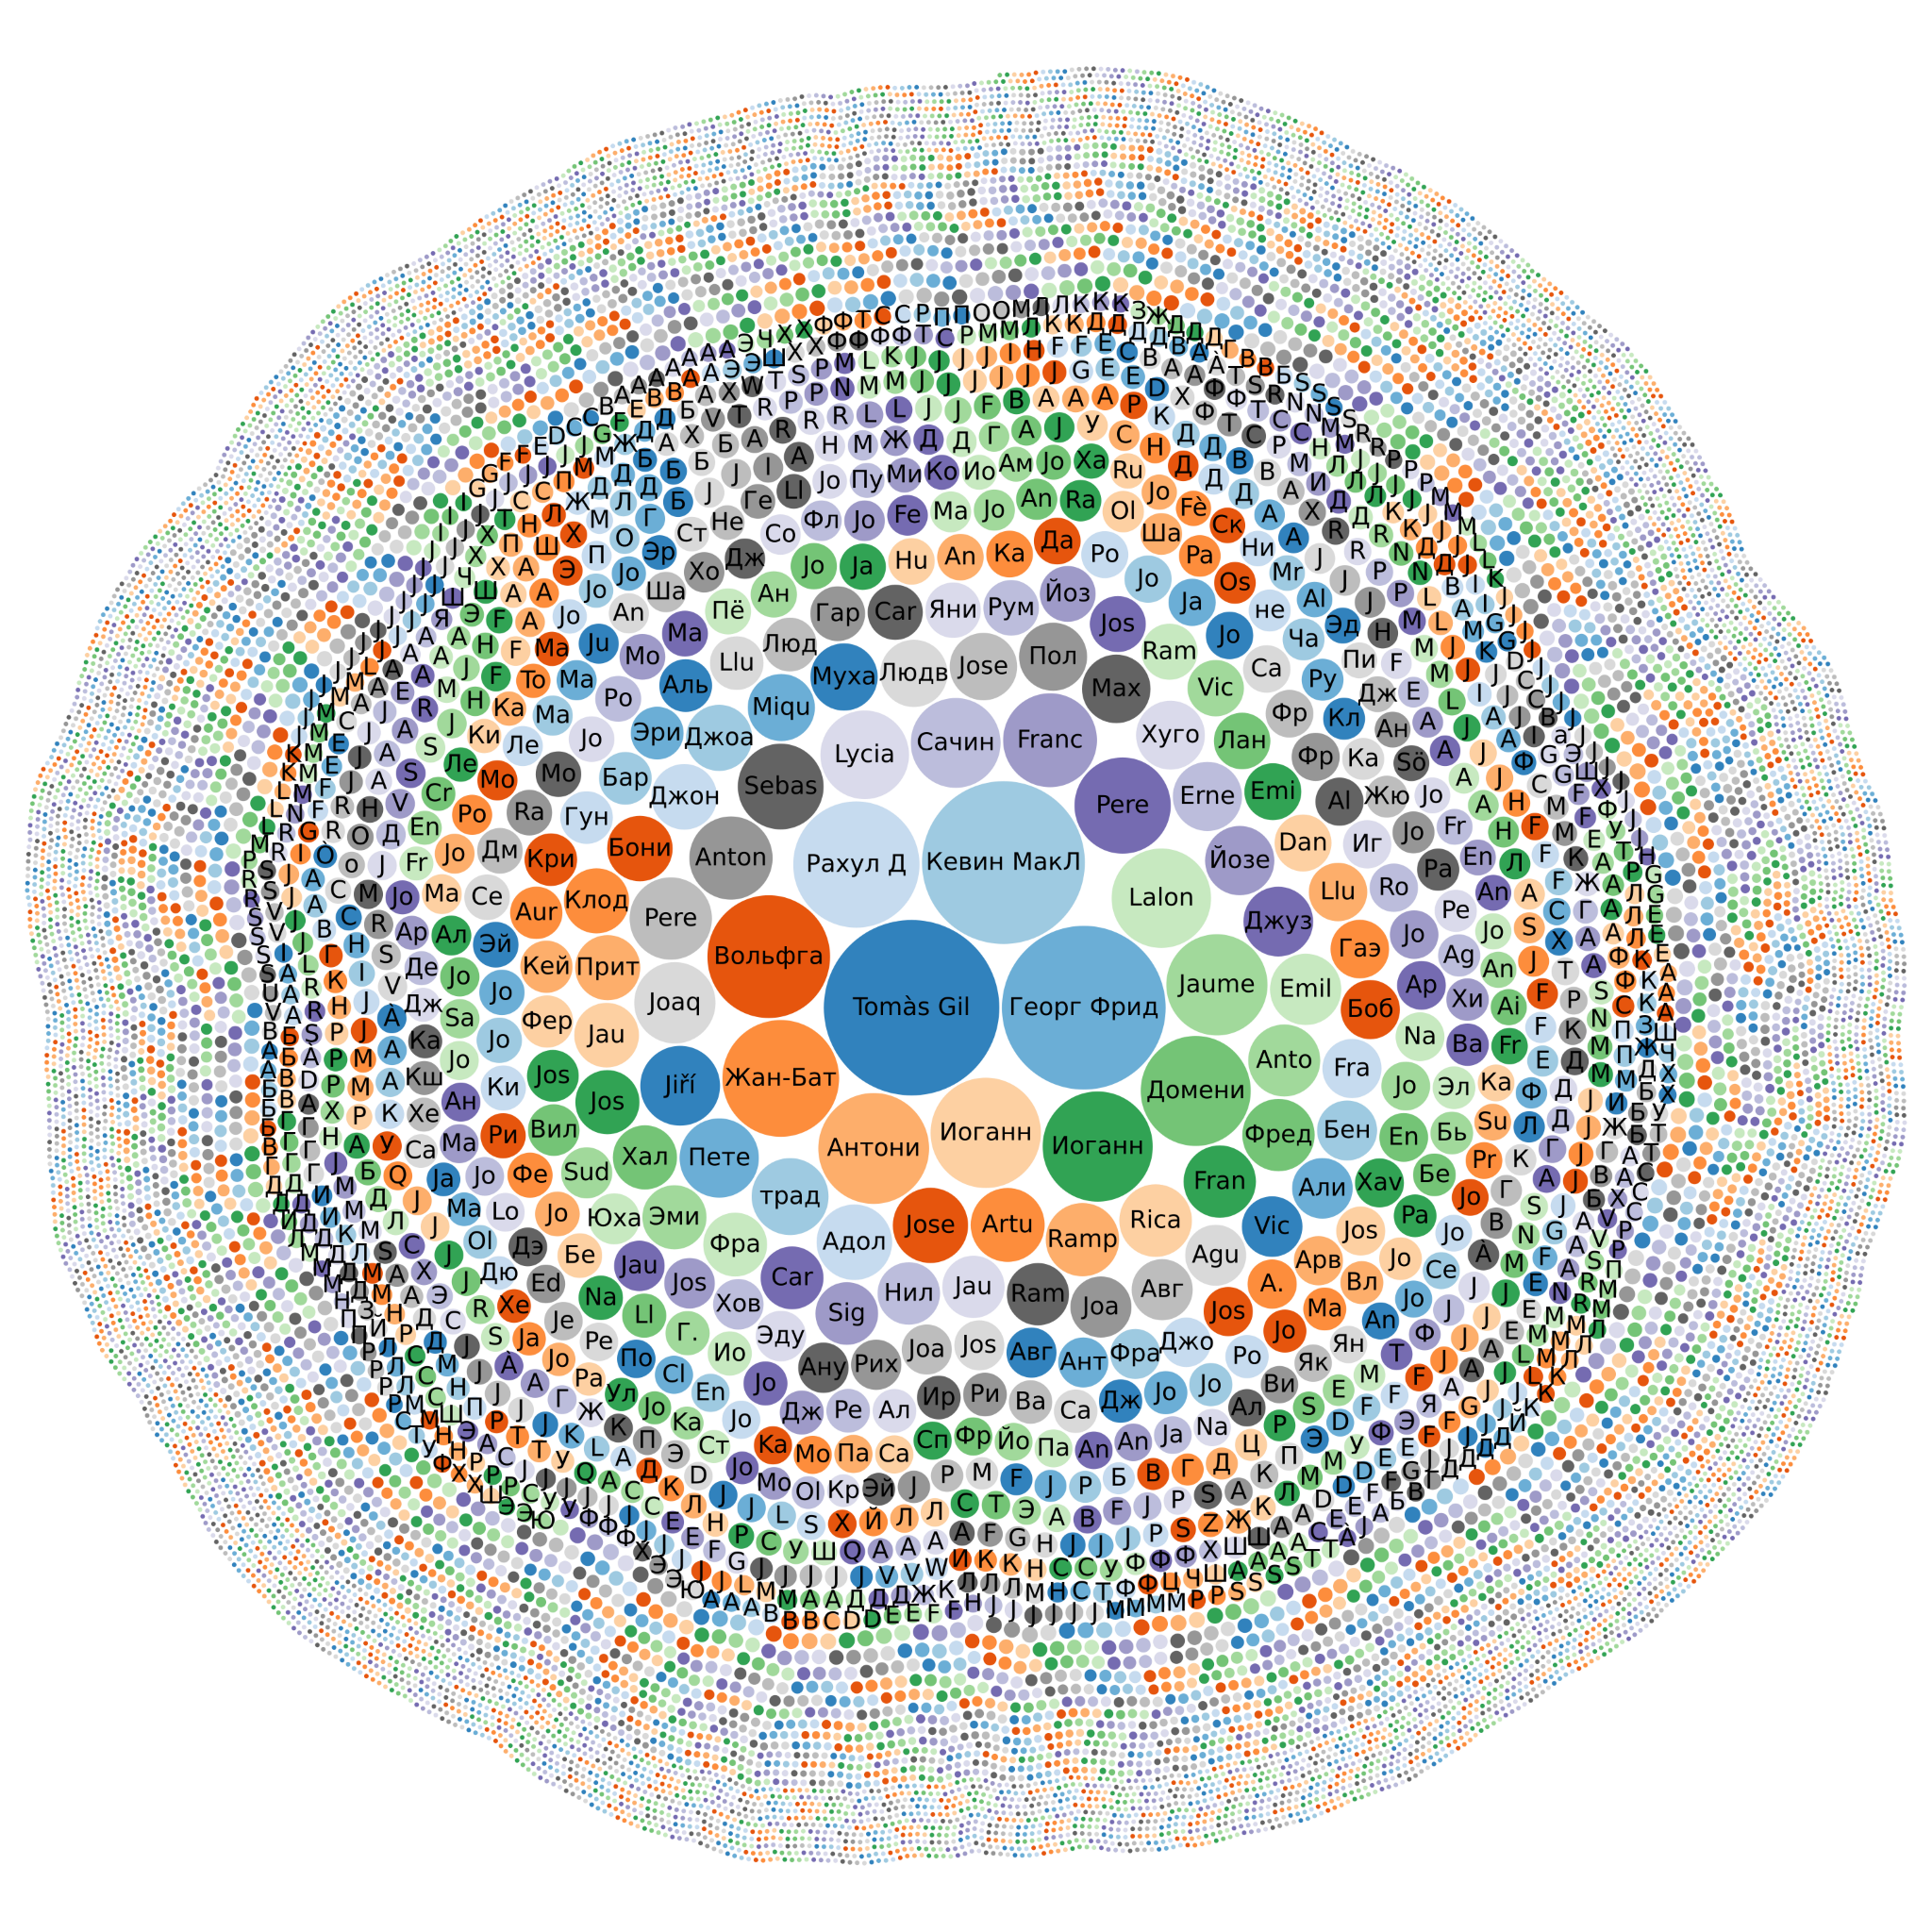
\includegraphics[width=\textwidth]{./chapter/musical_composition/Composer_of_musical_compositions_bubble_diagram.svg.png}
	\caption[Пузырьковая диаграмма композиторов по количеству написанных композиций за 2022 год]{Пузырьковая диаграмма композиторов по количеству написанных композиций за 2022 год}%
	\label{fig:bubbleChart2}%
\end{figure*}
\newpage


\subsection{Заполнение Викиданных}
Для того чтобы получить больше записей при выполнении скрипта для поиска музыкальных лакун в общественном достоянии, было решено заполнить свойство \wdProperty{86}{<<композитор>>} у объектов типа \wdqName{<<музыкальная композиция>>}{207628}.

Построим список всех музыкальных композиций с заполненным свойством \wdProperty{86}{<<композитор>>}.

\begin{lstlisting}[ language=SPARQL,
                    caption={\href{https://w.wiki/52VP}{ список всех музыкальных композиций с заполненным свойством <<композитор>>}\protect\footnotemark},
                    label=lst:Compositions_that_has_a_composer,
                    texcl 
                    ]
#Lists of compositions that has a composer
SELECT ?composition ?compositionLabel ?composer ?composerLabel 
WHERE {
  ?composition wdt:P31 wd:Q207628. # instance of composition
  ?composition wdt:P86 ?composer.  # composition has a composer
  SERVICE wikibase:label {bd:serviceParam wikibase:language "ru".}
}
}
\end{lstlisting}%
\footnotetext{Получено:\num{3965} записей на 2017 год. Ссылка на SPARQL-запрос: \href{https://w.wiki/56Sb}{https://w.wiki/56Sb}.}



\subsection{Упражнения}
\begin{enumerate}
\item Найти список музыкальных композиций, созданных во время эпохи классицизма (XVII—XVIII века).
Свойство: \wdProperty{571}{<<дата создания>>}.
\item Найти композитора, который написал больше симфоний чем остальные.
Свойства: \wdProperty{31}{<<экземпляр>>}, \wdProperty{86}{<<композитор>>}.
\item Построить гистограмму, на которой отображается количество музыкальных композиций группы The Beatles по году публикации.
Свойства: \wdProperty{175}{<<исполнитель>>}, \wdProperty{577}{<<дата публикации>>}.
\end{enumerate}
